\chapter{Divergences ultraviolettes et remède supersymétrique}

\lectureoverview{Avant d’introduire les mathématiques formelles de la supersymétrie, précisons le problème qu’elle est censée résoudre. Nous décrirons les divergences ultraviolettes dans l’espace des positions comme dans l’espace des impulsions, déduirons par analyse dimensionnelle le comportement à courte distance des propagateurs scalaires et fermioniques, puis estimerons les principales corrections de boucle à la masse d’un scalaire. Une boucle scalaire et une boucle fermionique ont la même dépendance quadratique au cutoff, mais des signes opposés. La supersymétrie devient particulièrement convaincante lorsqu’on se demande quel principe pourrait faire coïncider suffisamment leurs couplages, leurs multiplicités et leurs masses pour que cette annulation découle d’une structure plutôt que du hasard.}

\section{Pourquoi revenir aux divergences ?}

L’intention était d’aborder immédiatement les rouages de la supersymétrie. Il vaut toutefois mieux repousser l’abstraction d’un cours et reprendre les motivations depuis le début. L’exposé précédent sur les divergences et la renormalisation de la masse était rapide ; sans voir d’abord précisément ce qui doit être corrigé, la supersymétrie risque de sembler une invention mathématique arbitraire.

Les diagrammes de Feynman interviennent en physique des particules de deux façons étroitement liées. Le plus souvent, ils servent à organiser les amplitudes de diffusion. On précise les particules entrantes et sortantes, puis on somme les amplitudes représentées par tous les diagrammes de l’ordre requis. Ils servent aussi à construire un \emph{lagrangien effectif}. Ici, le mot ``effectif'' n’est pas un compliment qui signifierait « particulièrement réussi ». Il indique que la description est approchée : les détails inaccessibles à courte distance ont été éliminés ou intégrés, et leur influence est encodée dans les paramètres et les interactions qui subsistent.

Toute description de ce type possède un domaine de validité. On peut le spécifier au moyen d’une distance minimale jugée fiable, notée ici \(\delta\), ou d’une impulsion maximale jugée fiable,
\begin{equation}
\Lambda\sim \delta^{-1}.
\end{equation}
Ces deux cutoffs ne correspondent pas à des hypothèses distinctes. Ce sont deux descriptions, liées par transformation de Fourier, d’une même limite ultraviolette.

\section{Un propagateur, deux descriptions}

Le propagateur est l’amplitude associée à la création ou à l’insertion d’une particule en un point de l’espace-temps, puis à son annihilation ou à sa détection en un autre point. Notons ces deux points \(x^\mu\) et \(y^\mu\), et écrivons leur séparation sous la forme
\begin{equation}
\Delta^\mu=y^\mu-x^\mu.
\end{equation}
Nous réservons le symbole minuscule \(\delta\) au cutoff, afin de ne pas confondre la séparation avec le régulateur.

L’invariance par translation implique qu’un propagateur libre dépend de \(x\) et \(y\) uniquement par l’intermédiaire de \(\Delta\). Ce même objet peut être transformé de Fourier :
\begin{equation}
G(\Delta)
=\int\frac{d^4k}{(2\pi)^4}\,e^{-ik\cdot\Delta}\,\widetilde G(k).
\end{equation}

À la question ``Quels sont les conjugués de Fourier de la position ?'', posée à la salle, la réponse est : l’impulsion. Par conséquent, décrire une boucle dans l’espace des positions comme un propagateur qui revient à son point de départ équivaut, dans l’espace des impulsions, à intégrer sur toutes les impulsions susceptibles de circuler dans la boucle. Les règles dans l’espace des impulsions imposent de conserver l’impulsion à chaque sommet ; l’espace des positions rend plus transparent le raisonnement actuel sur le décompte des puissances.

Cette équivalence met en évidence le problème ultraviolet avant même tout calcul. Dans l’espace des positions, une boucle sonde la limite de coïncidence \(\Delta\to0\). Dans l’espace des impulsions, elle sonde la limite \(|k|\to\infty\). Une grande impulsion correspond à une courte longueur d’onde : une singularité à courte distance et une divergence à grande impulsion sont donc un même phénomène décrit dans des coordonnées différentes.

Le cours traite les classes de spin les plus simples : les champs scalaires, les champs fermioniques et, en toile de fond, les champs de jauge. Les scalaires ont un spin nul et sont représentés par un champ à une composante \(\phi(x)\). Lors de l’enregistrement du cours, en 2010, le Higgs n’avait pas encore été découvert et était présenté comme le principal scalaire attendu en physique des particules. Ce contexte historique explique l’expression facétieuse ``higgly-wiggly'' : le champ était d’une grande importance physique, mais n’avait pas encore été établi expérimentalement.

Pour un champ scalaire réel, le propagateur peut s’écrire schématiquement
\begin{equation}
G_\phi(x,y)=\expect{0|T\!\left\{\phi(x)\phi(y)\right\}|0}
=G_\phi(\Delta).
\end{equation}
La convention d’ordonnancement temporel et la normalisation n’importeront pas pour notre décompte des puissances. Le point essentiel est que les deux insertions du champ décrivent la création en un point et l’annihilation en l’autre.

\begin{classroomqa}
\audiencequestion{\(x\) et \(y\) sont-ils des points de l’espace ou de l’espace-temps ? \lecturetimestamp{00:09:31}}
\lecturerresponse{Ce sont des points de l’espace-temps. Chacun est un quadrivecteur. Le propagateur dépend donc de leur séparation quadridimensionnelle et, dans un vide invariant de Lorentz, de l’intervalle invariant correspondant.}
\end{classroomqa}

Une particule de spin un demi est décrite par un champ de Dirac \(\psi_i(x)\). L’indice \(i\) est un indice de spineur, et non une composante spatiale ; le propagateur est donc une matrice :
\begin{equation}
S_{ij}(x,y)=\expect{0|T\!\left\{\psi_i(x)\bar\psi_j(y)\right\}|0}
=S_{ij}(\Delta).
\end{equation}

Une question posée à la salle permet de préciser le nombre de composantes : un champ de Dirac en quatre dimensions en possède quatre, complexes. Un champ de Weyl sans masse peut être décrit au moyen de deux composantes complexes ; les champs de chiralités gauche et droite peuvent donc être traités séparément. Pour le présent raisonnement dimensionnel, seule importe l’existence de la structure matricielle de spineur.

Puisque \(S_{ij}\) est une matrice \(4\times4\), on peut la développer dans la base des matrices de Dirac. Nous omettrons d’abord ces indices et les rétablirons lorsqu’ils seront nécessaires. Cela ne signifie pas que la structure matricielle soit absente : c’est une simplification délibérée, le temps d’établir la loi de puissance ultraviolette.

\begin{classroomqa}
\audiencequestion{Dans quels cas le champ conjugué, ou adjoint, doit-il apparaître dans un propagateur ? \lecturetimestamp{00:14:06}}
\lecturerresponse{Dans cette discussion schématique d’un scalaire réel neutre, le même champ contient les opérateurs de création et d’annihilation ; il n’est donc pas nécessaire de faire intervenir un champ adjoint distinct. Pour un champ chargé, il faut distinguer les opérateurs de particule et d’antiparticule. Ainsi, \(\psi\), \(\psi^\dagger\) et, de manière covariante, \(\bar\psi=\psi^\dagger\gamma^0\) jouent des rôles différents pour un électron.}
\end{classroomqa}

La particule de Higgs physique est neutre, bien que le champ de Higgs sous-jacent du Modèle standard soit un doublet électrofaible. Le cours prend comme modèle local un scalaire réel neutre ; cette simplification suffit pour l’estimation ultraviolette.\editorialnote{Cette distinction évite de prendre l’exemple schématique du scalaire réel pour un énoncé complet sur le multiplet de Higgs électrofaible.}

\section{Unités naturelles et dimension d’un champ scalaire}

Posons \(\hbar=c=1\). La longueur et le temps ont alors la même unité, tandis que l’énergie, la masse et l’impulsion ont l’unité de l’inverse d’une longueur :
\begin{equation}
[m]=[E]=[p]=L^{-1}.
\end{equation}
L’action intervient dans la phase \(e^{iS}\) ; elle est donc sans dimension. Une action scalaire représentative en quatre dimensions d’espace-temps est
\begin{equation}
S_\phi=\int d^4x\left[
\frac12\partial_\mu\phi\,\partial^\mu\phi
-\frac12m^2\phi^2
-\frac{\lambda}{4!}\phi^4
+\cdots\right].
\end{equation}
Les facteurs conventionnels \(1/2\) et \(1/4!\) n’ont pas d’incidence sur l’analyse dimensionnelle.

Commençons par le terme cinétique. Puisque \([d^4x]=L^4\) et \([\partial_\mu]=L^{-1}\), l’absence de dimension impose
\begin{align}
1
&=L^4\left(L^{-1}[\phi]\right)^2,\\
[\phi]&=L^{-1}.
\end{align}
Le terme de masse fournit une vérification :
\begin{equation}
L^4[m^2][\phi^2]
=L^4L^{-2}L^{-2}=1.
\end{equation}

La question suivante posée à la salle porte sur la dimension du couplage quartique. En quatre dimensions d’espace-temps, il est sans dimension :
\begin{equation}
L^4[\lambda][\phi]^4=L^4[\lambda]L^{-4}=1
\quad\Longrightarrow\quad [\lambda]=L^0.
\end{equation}
Cela confère à l’interaction \(\phi^4\) un statut particulier en quatre dimensions. Les dimensions de \(\phi^6\) et des interactions d’ordre supérieur se déduisent de la même façon, mais leurs couplages comportent des puissances négatives de la masse, signe qu’ils jouent un rôle plus restreint dans une théorie effective.

Les dimensions des champs nous indiquent donc déjà quelles interactions peuvent avoir des coefficients sans dimension. La même méthode permettra de déterminer les deux propagateurs ainsi que le couplage de Yukawa, sans calculer d’intégrale de Feynman détaillée.

\section{Le propagateur scalaire à courte distance}

Considérons d’abord un scalaire sans masse. Il n’existe aucune échelle de longueur intrinsèque ; la seule échelle disponible est la séparation \(\Delta\). L’invariance par translation ne laisse subsister que \(\Delta\), l’invariance de Lorentz réduit la dépendance à sa norme invariante, et le produit de deux champs scalaires est de dimension \(L^{-2}\). À une constante numérique près,
\begin{equation}
G_0(\Delta)\sim\frac{1}{\Delta^2}.
\end{equation}
Un raisonnement dimensionnel seul ne permet pas de fixer des facteurs tels que \(4\pi^2\).

Une masse introduit la longueur de Compton \(m^{-1}\). Son effet se comprend le plus facilement à partir de la relation de dispersion
\begin{equation}
E=\sqrt{\bm p^{,2}+m^2},
\qquad
E=|\bm p|\quad(m=0).
\end{equation}
Lorsque \(|\bm p|\gg m\), la masse est négligeable. Comme les grandes impulsions sondent les courtes distances, le propagateur massif doit tendre vers le comportement \(1/\Delta^2\) sans masse lorsque \(\Delta\to0\). Aux distances très supérieures à \(m^{-1}\), la propagation est supprimée. Le cours représente schématiquement ce fait par
\begin{equation}
G_m(\Delta)\sim \frac{e^{-m|\Delta|}}{\Delta^2}.
\end{equation}
Il ne s’agit délibérément pas d’une formule exacte. En espace euclidien à quatre dimensions, le propagateur libre exact est proportionnel à \(mK_1(mr)/r\), avec \(r=|\Delta|\) ; il présente la même singularité ultraviolette \(1/r^2\) et décroît exponentiellement à grande distance, avec un préfacteur en loi de puissance.\editorialnote{La forme faisant intervenir la fonction de Bessel donne la complétion précise habituelle de l’exponentielle schématique du cours ; elle n’est pas nécessaire pour son raisonnement sur le décompte des puissances.}

La leçon essentielle est simple : la masse atténue la propagation à grande distance, mais ne supprime pas la singularité au point de coïncidence. Au voisinage suffisamment proche d’un point, toute masse finie devient négligeable.

\section{Le tadpole scalaire et le réglage fin}

L’interaction quartique \(\lambda\phi^4\) produit un sommet à quatre lignes. Relions deux de ses branches entre elles et laissons deux branches scalaires externes. Le diagramme en tadpole qui en résulte corrige le coefficient de \(\phi^2\), et donc la masse au carré du scalaire.

L’image conservée montre exactement le passage de l’analyse dimensionnelle à cette correction de boucle. La relation de dispersion reste visible à gauche, l’action scalaire et la dimension du champ le sont en partie à droite, et le petit tadpole vient d’apparaître au centre.

\begin{figure}[H]
\centering
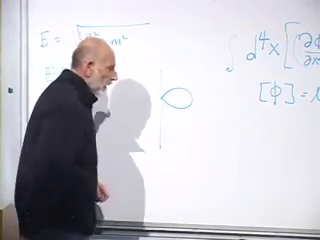
\includegraphics[width=0.72\textwidth]{lecture_03_figure_02.png}
\lectureframe{00:28:30.560}

\medskip
\begin{tikzpicture}[line width=0.8pt,scale=1.0]
  \draw[dashed] (-2.6,0) -- (0,0) -- (2.6,0);
  \fill (0,0) circle (0.055);
  \draw (0,0) .. controls (-0.85,0.7) and (-0.85,1.6) .. (0,1.6)
                .. controls (0.85,1.6) and (0.85,0.7) .. (0,0);
\end{tikzpicture}
\caption{Le tableau au moment du passage à l’auto-énergie scalaire, suivi d’un schéma prudent de la topologie du tadpole. La capture montre clairement la boucle, les formules de l’énergie relativiste et de l’énergie sans masse, ainsi qu’une partie de l’action ; elle ne permet pas d’affirmer que les coefficients et les légendes masqués sont visibles.}
\end{figure}

Au sommet, le scalaire peut être absorbé puis réémis, tandis que les deux autres branches se propagent du point à lui-même. À des facteurs numériques et combinatoires près, la correction vaut
\begin{equation}
\delta m_\phi^2\sim \lambda G_\phi(0).
\end{equation}
Dans l’approximation du continuum, le propagateur au point de coïncidence est infini. Une théorie effective ne prétend pas être valable à une distance arbitrairement courte ; imposons donc \(|\Delta|\geq\delta\). On obtient alors
\begin{equation}
G_\phi(0)\longrightarrow G_\phi(\delta)sim\frac{1}{\delta^2},
\qquad
\delta m_\phi^2\sim\frac{\lambda}{\delta^2}sim\lambda\Lambda^2.
\end{equation}
On parle de divergence quadratique car elle comporte deux puissances du cutoff en impulsion. L’intégration dans l’espace des impulsions conduit à la même conclusion : la contribution excessive provient des impulsions de boucle arbitrairement grandes. Que l’échelle minimale soit finalement fixée par la grande unification, la gravité quantique ou quelque chose qui reste à imaginer ne change rien au diagnostic de la théorie effective.

C’est un problème de réglage fin. Si \(\delta\) est extrêmement petit et si \(\lambda\) n’est pas extraordinairement minuscule, la correction radiative est bien supérieure à la masse au carré du scalaire observée à basse énergie. Le coefficient nu et la correction de boucle doivent alors s’annuler avec un nombre invraisemblable de chiffres de précision :
\begin{equation}
m_{\mathrm{physical}}^2
=m_{\mathrm{bare}}^2+\delta m_\phi^2.
\end{equation}
Le propagateur massif ne résout pas le problème. Aux distances responsables de la divergence, \(e^{-m|\Delta|}\simeq1\). La boucle ultraviolette a oublié la masse bien avant d’atteindre le cutoff.

\section{Dimensions du fermion et son propagateur}

Reprenons maintenant la même analyse dimensionnelle pour un fermion de Dirac. Son action libre est
\begin{equation}
S_\psi=\int d^4x\,
\bar\psi\left(i\gamma^\mu\partial_\mu-m\right)\psi.
\end{equation}
Les matrices gamma sont numériques et sans dimension. Comme le terme cinétique ne contient qu’une seule dérivée,
\begin{align}
1
&=L^4[\bar\psi]L^{-1}[\psi],\\
[\psi]=[\bar\psi]&=L^{-3/2}.
\end{align}
Les puissances demi-entières n’ont rien d’inquiétant ; les fermions font apparaître des moitiés en de nombreux endroits.

\begin{classroomqa}
\audiencequestion{Ne serait-il pas plus simple de déduire \([\psi]\) du terme de masse ? \lecturetimestamp{00:36:02}}
\lecturerresponse{Oui. Le terme de masse donne \(L^4L^{-1}[\bar\psi\psi]=1\), d’où \([\bar\psi\psi]=L^{-3}\) et \([\psi]=L^{-3/2}\). Nous avons commencé par la dérivation cinétique parce qu’elle reste pertinente dans la théorie sans masse et montre pourquoi la masse du fermion apparaît comme \(m\), et non comme \(m^2\).}
\end{classroomqa}

Deux champs fermioniques sont de dimension \(L^{-3}\) ; le raccourci dimensionnel employé dans le cours pour le propagateur sans masse est donc
\begin{equation}
S(\Delta)\sim\frac{1}{|\Delta|^3}.
\end{equation}
Rétablir sa structure matricielle donne au numérateur la forme plus précise exigée par la covariance de Lorentz :
\begin{equation}
S_{ij}(\Delta)
\propto
\frac{\left(\gamma_\mu\Delta^\mu\right)_{ij}}
{\left(\Delta^2\right)^2}.
\end{equation}
Le numérateur apporte une puissance de longueur et le dénominateur contient donc quatre puissances de l’intervalle ; la dimension nette reste \(L^{-3}\). Comme pour le scalaire, une masse fermionique supprime le propagateur à grande distance, mais ne modifie pas cette loi d’échelle à courte distance.

\section{Pourquoi une boucle fermionique fermée est négative}

Nous pouvons maintenant nous demander si un diagramme fermionique pourrait annuler la mauvaise auto-énergie bosonique. Le tadpole scalaire a un signe positif, à des facteurs numériques positifs près, tels que des puissances de \(\pi\) et des coefficients combinatoires. Une boucle fermionique fermée porte le signe opposé.

\begin{classroomqa}
\audiencequestion{Le signe moins de la boucle fermionique est-il lié à la discussion précédente sur une rotation complète ? \lecturetimestamp{00:40:21}}
\lecturerresponse{Il relève de la même structure de signes fermioniques, mais la démonstration utile ici repose sur l’antisymétrie par échange, plutôt que sur l’orientation géométrique d’une boucle. Coupons deux boucles, échangeons les particules identiques, puis reconnectons-les. L’échange transforme deux boucles en une seule et introduit un signe moins pour les fermions uniquement.}
\end{classroomqa}

Il vaut la peine de donner le raisonnement en détail. Supposons qu’un diagramme à une boucle ait le signe \(\sigma\), positif ou négatif. Deux boucles identiques et déconnectées ont le signe
\begin{equation}
\sigma^2=+1.
\end{equation}
Coupons simultanément les deux boucles. Deux particules identiques se propagent alors entre les points de coupure. Leur fonction d’onde ordinaire à deux particules est symétrique pour des bosons et antisymétrique pour des fermions :
\begin{align}
\Psi_B(x_1,x_2)&=+\Psi_B(x_2,x_1),\\
\Psi_F(x_1,x_2)&=-\Psi_F(x_2,x_1).
\end{align}
L’antisymétrie explique aussi le principe de Pauli : si l’on place les deux fermions dans le même état, l’échange ne change rien physiquement, mais doit inverser la fonction d’onde, qui doit donc s’annuler.

Reconnectons les lignes coupées après avoir échangé les deux particules. Du point de vue topologique, les deux boucles n’en forment plus qu’une. L’amplitude à deux boucles avant l’échange était positive. L’échange la laisse positive pour les bosons et en inverse le signe pour les fermions. Par conséquent,
\begin{equation}
\begin{aligned}
\operatorname{sign}(\text{closed boson loop})&=+1,\\
\operatorname{sign}(\text{closed fermion loop})&=-1.
\end{aligned}
\end{equation}
La conclusion est générale : chaque boucle fermionique fermée indépendante apporte un facteur \(-1\).

\section{La boucle de Yukawa}

Revenons à la masse du scalaire. Un boson ne peut pas se transformer en un fermion unique, car cela changerait la parité du nombre fermionique. La correction fermionique la plus simple consiste à faire se scinder le scalaire en une paire fermion-antifermion, qui parcourt une boucle avant de se recombiner. L’interaction est un couplage de Yukawa,
\begin{equation}
\mathcal L_Y=-g\phi\bar\psi\psi.
\end{equation}
Dans le cas du Higgs, les fermions peuvent être des quarks ou des leptons. Il y a deux points d’interaction, donc deux facteurs de \(g\).

Le tadpole scalaire impliquait un seul point, dont on pouvait fixer la position globale puisque l’invariance par translation ne fournit que le volume de l’espace-temps. La boucle de Yukawa implique deux points. On peut fixer l’un d’eux, ou, de façon équivalente, leur position moyenne, mais il faut intégrer sur leur séparation relative \(\Delta\). Chaque propagateur fermionique apporte le facteur à courte distance \(1/|\Delta|^3\), donc
\begin{equation}
\delta m_{\phi,F}^2
\sim
-g^2\int_{|\Delta|\geq\delta}d^4\Delta\,
\frac{1}{|\Delta|^6}.
\end{equation}

Après avoir écrit les deux propagateurs, l’intégrale sur la séparation et les deux couplages, le cours demande à la salle un dernier facteur. La réponse est le signe moins. Les deux propagateurs se referment en une boucle fermionique ; toute l’intégrale à courte distance, positive par ailleurs, est donc multipliée par \(-1\).

L’analyse dimensionnelle suffit déjà à déterminer la divergence. \(d^4\Delta\) fournit quatre puissances de longueur, tandis que le dénominateur en comporte six ; la seule échelle de longueur qui reste est celle du cutoff :
\begin{equation}
\int_{|\Delta|\geq\delta}
\frac{d^4\Delta}{|\Delta|^6}
\sim\frac{1}{\delta^2}.
\end{equation}
En coordonnées radiales euclidiennes à quatre dimensions, on peut l’expliciter :
\begin{equation}
\int_{\delta}^{R}d^4\Delta\,\frac{1}{|\Delta|^6}
=2\pi^2\int_{\delta}^{R}dr\,\frac{r^3}{r^6}
=\pi^2\left(\frac{1}{\delta^2}-\frac{1}{R^2}\right).
\end{equation}
Les traces de spineurs et les normalisations des propagateurs modifient le coefficient, mais pas la dépendance quadratique au cutoff.\editorialnote{L’intégrale radiale est une forme explicite classique de l’estimation dimensionnelle donnée dans le cours. Elle est écrite en distance euclidienne, où la positivité et le décompte des puissances ultraviolettes sont transparents.}

\begin{classroomqa}
\audiencequestion{Le choix des bornes d’intégration ou leur inversion peut-il changer le signe ? \lecturetimestamp{00:51:06}}
\lecturerresponse{Non. Il ne s’agit pas d’une intégrale unidimensionnelle orientée dont les bornes produiraient le signe physique. C’est une intégrale sur quatre composantes, ou, plus simplement, sur une mesure radiale positive. Sa contribution ultraviolette est positive. Le signe négatif provient uniquement de la boucle fermionique fermée.}
\end{classroomqa}

\begin{classroomqa}
\audiencequestion{Quelle est la dimension du couplage de Yukawa \(g\) ? \lecturetimestamp{00:51:51}}
\lecturerresponse{Il est sans dimension en quatre dimensions. Puisque \([\phi]=L^{-1}\) et \([\bar\psi\psi]=L^{-3}\), le produit \(\phi\bar\psi\psi\) est de dimension \(L^{-4}\), exactement compensée par \(d^4x\).}
\end{classroomqa}

La principale correction fermionique est donc
\begin{equation}
\delta m_{\phi,F}^2
\sim -C_F\frac{g^2}{\delta^2}
=-C_Fg^2\Lambda^2,
\end{equation}
où \(C_F>0\) regroupe des facteurs numériques, de spin et de multiplicité. La boucle scalaire prend la forme correspondante
\begin{equation}
\delta m_{\phi,B}^2
\sim+C_B\frac{\lambda}{\delta^2}
=+C_B\lambda\Lambda^2.
\end{equation}
Nous n’avons pas encore résolu le problème du réglage fin, mais nous avons trouvé un élément indispensable : une contribution de même degré ultraviolet et de signe opposé.

\section{Conditions nécessaires à l’annulation}

Ce serait une coïncidence extraordinaire que des couplages sans lien entre eux vérifient
\begin{equation}
C_B\lambda=C_Fg^2
\end{equation}
avec exactement la précision exigée par une grande hiérarchie d’échelles. Le cours résume cela par \(g^2=\lambda\), en omettant les facteurs dépendant des conventions et les facteurs de multiplicité. Une véritable solution exige une structure mathématique qui impose cette relation au lieu de simplement la permettre.

C’est ce qui motive la supersymétrie. Elle relie bosons et fermions et restreint leurs couplages à des combinaisons qui provoquent l’annulation de nombreux termes divergents autrement dangereux. L’annulation se reproduit alors dans plusieurs diagrammes parce qu’elle découle d’une symétrie, et non d’un ajustement des paramètres boucle après boucle.

L’égalité des masses importe également. Si les masses du boson et du fermion sont identiques, leurs propagateurs complets peuvent être appariés au mieux. Si elles diffèrent légèrement, les réponses complètes et finies ne s’annulent pas exactement, car les propagateurs diffèrent à des distances comparables à leurs longueurs de Compton. Leurs comportements asymptotiques communs à courte distance peuvent néanmoins annuler la partie divergente :
\begin{equation}
\mathcal I_B(\Delta)-\mathcal I_F(\Delta)
\quad\hbox{may be finite as}\quad \Delta\to0,
\end{equation}
où \(\mathcal I_B\) et \(\mathcal I_F\) désignent les intégrandes complets des boucles bosonique et fermionique, après prise en compte des sommets, des numérateurs et des multiplicités. On ne soustrait pas directement les propagateurs eux-mêmes, qui sont de dimensions différentes. Même lorsque les termes ultraviolets s’annulent, il peut subsister une contribution finie. C’est ce qui ouvre la voie à une supersymétrie approchée ou brisée. L’égalité exacte produit l’annulation la plus nette ; une brisure suffisamment contrôlée peut tout de même éliminer la catastrophe ultraviolette tout en laissant des écarts de masse observables.

Nous sommes ainsi parvenus à la supersymétrie sans encore en écrire l’algèbre. Le raisonnement est complet :
\begin{equation}
\begin{gathered}
G_\phi(\Delta)\sim \Delta^{-2},
\qquad
\delta m_{\phi,B}^2\sim+C_B\lambda\Lambda^2,\\[0.4em]
S_\psi(\Delta)\sim \Delta^{-3},
\qquad
\delta m_{\phi,F}^2\sim-C_Fg^2\Lambda^2,\\[0.4em]
\text{symmetry-enforced matching}\\
\Longrightarrow\quad
\text{quadratic divergences cancel}.
\end{gathered}
\end{equation}
Il reste à comprendre le principe abstrait de symétrie qui impose ces relations et à examiner des exemples concrets de son action.
